\section{Algorithm Implementation}
In this section the implementation of the baseline algorithm is described, additionally a flowchart is established as an illustration of the flow through code resulting from the implementation of the algorithm. 
The baseline algorithm consist of three main stages, an initialization, COV-DL for recovery of $\textbf{A}$ and lastly M-SBL for recovery of $\textbf{X}$. 
Consider figure \ref{fig:flow}. 
Each stage of the algorithm is illustrated within one horizontal row of the flow diagram, furthermore the input and output are placed in their own row.    

\begin{figure}[H]
\centering
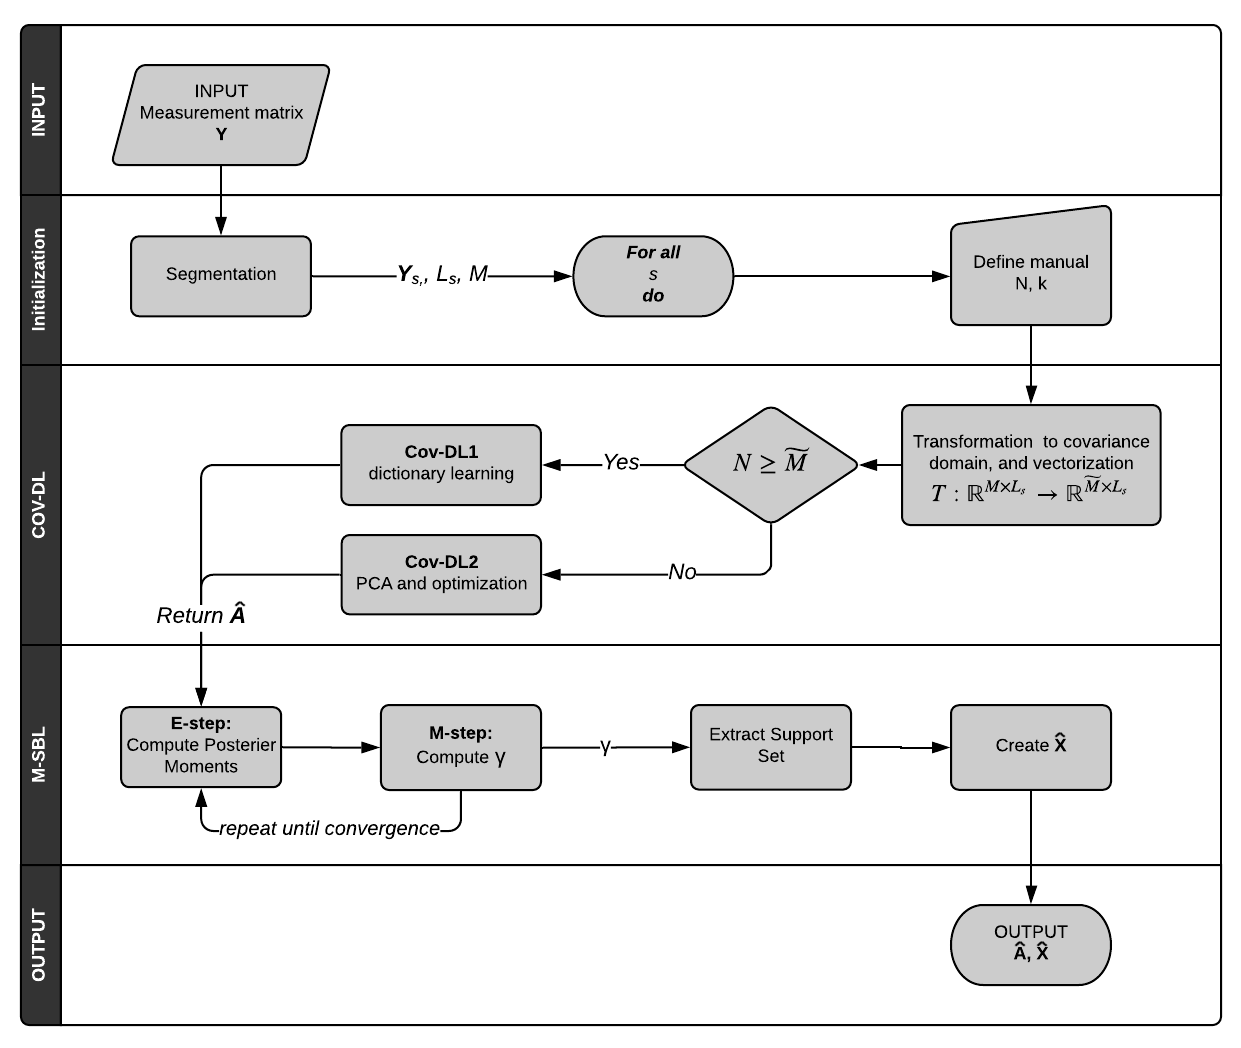
\includegraphics[scale=0.8]{figures/ch_6/baseline_flowchart.png}
\caption{Flowchart illustrating the implementation of the baseline algorithm.}
\label{fig:flow}
\end{figure}
\noindent
\todo{indsæt hat på gamma, X og A i flowchart}

The input consist of the data matrix $\textbf{Y}\in \mathbb{R}^{M\times L}$, along with the corresponding sample frequency. 
Within the initialization stage the input data go through a segmentation as described in subsection \ref{seg_segmentation}. The length of the segments are predefined by a time interval $t$ in seconds such that $L_{s} = tf$. 
Each segment s is now specified by the data matrix $\textbf{Y}\in \mathbb{R}^{M \times L_{s}}$.
After the segmentation a for loop is constructed such that for every segments s the remaining to stages of the algorithm are performed. 
For each segment $N$ and $k$ are manually defined, this definition are either known in advance from the data or in the case of real EEG measurement they are unknown and a qualified guess must be made\todo{the manual input is an issue time wise when running over many segments, so the input should be made in advance}.
With one data segment and corresponding specifications of the expected number of active sources the second stage of the algorithm are initialised, recovery of $\textbf{A}$.
The implementation of COV-DL stage follows algorithm \ref{alg:Cov1} of section \ref{seg:alg_cov} closely thus only the main steps are illustrated on the flow digram.
First the data matrix $\textbf{Y}_s$ are transformed to the covariance domain and then vectorised, resulting in an extension of the dimensionality from $M$ of $\widetilde{M}=\frac{M(M+1)}{2}$\todo{should we define new number of "samples" as well?}.
Next, the estimation of $\textbf{A}$ is performed from either COV-DL1 or COV-DL2 depending on the relation between $M$ and $N$, as descried respectively in section \ref{sec:cov1} and \ref{sec:over_det}.
The estimate $\hat{\textbf{A}}$ serve as the input to the next stage, M-SBL for recovering of $\textbf{X}$, along with the original data segment $\textbf{Y}_s$. The last stage of the algorithm consist of the iterative EM algorithm for maximising the marginal likelihood \eqref{eq:likelihood} with respect to $\boldsymbol{\gamma}$, which is the hyperparameter from which $\textbf{X}$ can be determined as described in section \ref{seg:M_sblalg}. Lastly the output of the baseline algorithm $\hat{\textbf{X}}$ and $\hat{\textbf{A}}$ is illustrated on the flowchart.

\subsection{Coding Practice}
The implementation of the baseline algorithm in performed in Python 3.7. The software and guide to run the scripts are available through appendix \ref{App:code}.

The practical implementation process are based on module development. The established model and the three main stages of the algorithm makes a superior system design. For each stage the necessary tasks are identified and divided into smaller modules. For each module the task is specified and the an algorithm are established and implemented. This is followed by a test of the module and possible modifications until the task is performed without error. 
Due to the time limitation of this project the software was developed along side the dynamic research process. Thus the specifications to some modules have been redefined and hence the modification process are repeated. 
Finally the modules are united. First to one main stage for which tests are performed, and lastly all the main staged are united to the resulting baseline algorithm.

The software are based function definitions for which docstrings is used, following Numpy docstring format\footnote{\url{https://numpydoc.readthedocs.io/en/latest/}} allowing insight
into the structure and thoughts behind the different software elements.

The verification test and performance test each of the main stages, COV-DL and M-SBL are described later in this chapter, followed by tests of the final base line algorithm. 

